% Project FLASH V1: IEEE conference paper (IEEEtran, two-column).
% Self-contained: the references are embedded below, so no BibTeX run is needed.
% Build in this folder (figures/ next to this file):  pdflatex flash_v1  (run twice)
% Every number traces to the repository: PROJECT_FLASH_REPORT.md cites the source file of each,
% and the derived ones are recomputed by tools/make_report_figures.py into
% docs/figures/derived_numbers.json. The plots in figures/ are written by that script.
\documentclass[conference]{IEEEtran}
\usepackage[T1]{fontenc}
\usepackage{amsmath,amssymb}
\usepackage{graphicx}
\usepackage{booktabs}
\usepackage[hyphens]{url}
\usepackage{cite}
\usepackage{tikz}
\usetikzlibrary{arrows.meta,fit,positioning}
\usepackage[hidelinks]{hyperref}

\newcommand{\meas}{\textsuperscript{M}}   % Measured (tables only)
\newcommand{\deriv}{\textsuperscript{D}}  % Derived (tables only)
\newcommand{\synest}{\textsuperscript{S}} % Synthesis estimate (tables only)
\newcommand{\code}[1]{\texttt{#1}}

\begin{document}

\title{FLASH: A Bit-Exact Integer CNN for Offline Chest X-Ray Pneumonia Screening on a Low-Cost Zynq-7020}

\author{\IEEEauthorblockN{Karthikeya Reddy and Yashwant Rajesh}
\IEEEauthorblockA{BITS Pilani, Hyderabad Campus, India}}

\maketitle

\begin{abstract}
FLASH is a pneumonia screener whose complete convolutional neural network runs in the
programmable logic of a low-cost Zynq-7020 (PYNQ-Z2 board) and reproduces an independent integer
reference model bit for bit. The network is trained directly in integer units on 224$\times$224
chest radiographs from the RSNA Pneumonia Detection dataset. It has five stride-2 3$\times$3
convolutions, global average pooling and a 64$\to$2 classifier, with 47,602 parameters and 12.19
million multiply-accumulates (MACs) per image. A single convolution engine, configured at run
time by a 128-bit descriptor per layer, executes the same Verilog at 28$\times$28 and
224$\times$224. Three bit-exact links connect the trained network, a NumPy golden model, RTL
simulation and the board. On the board, all 244 verification images match the reference in
logit0, logit1, margin and decision, on three bitstreams. At 66.67\,MHz an image takes
182.94\,ms, 99.97\% of the engine's one-MAC-per-clock peak. On 4,003 held-out patients the model
reaches an AUROC of 0.8229 (95\% CI 0.8083--0.8379). The first board run produced no bit-exact
result (0/244) although 234 of 244 decisions agreed with the reference. We located the cause
offline from the board's logits, a data-width mismatch in the processor's memory bridge, and
confirmed it by changing one register bit, which restored 244/244. A subgroup analysis exposes two
failure modes: low specificity on radiographs with other abnormalities, and partial reliance on
the radiographic projection. FLASH is a research prototype and is not a medical device.
\end{abstract}

\begin{IEEEkeywords}
FPGA, CNN accelerator, integer inference, chest X-ray, pneumonia, verification, medical AI
\end{IEEEkeywords}

% ------------------------------------------------------------------------------------------
\section{Introduction}

Pneumonia killed 740,180 children under five in 2019, 14\% of all deaths in that age group
\cite{who2022pneumonia}. A chest radiograph is the usual confirmation, but it needs a reader,
and where readers are scarce a film can wait a long time for its report. Deep networks can read
chest radiographs \cite{wang2017chestxray8,rajpurkar2017chexnet}, but they usually run on a
server, which needs connectivity and sends images off site. A small device that reads the film
where it is taken, without a network connection, and gives an immediate first opinion could help
a clinician decide which films to read first.

We use an FPGA because the circuit computes the same integers as the validated reference model
on every run, without an operating system or a floating-point library in between. The hardware
and the reference can therefore be compared exactly, output by output, and an integration fault
appears as a difference in a 32-bit integer.

This paper describes FLASH V1, a research prototype on the PYNQ-Z2 board, and makes four
contributions:
\begin{enumerate}
\item A bit-exact integer co-design and verification flow, from training to golden model to RTL
to board, at 224$\times$224 on a low-cost Zynq-7020 (Sections~\ref{sec:model} and
\ref{sec:verif}).
\item A resolution-agnostic convolution engine driven by a layer table, which ran 28$\times$28
and 224$\times$224 with the same Verilog (Section~\ref{sec:hw}).
\item A board-only integration fault that was localised offline from the logits and confirmed by
intervention. Decision-level agreement was 234/244 while no logit was correct, so only the
logit-level comparison detected it (Section~\ref{sec:afi}).
\item A subgroup analysis exposing two failure modes: confusion of other lung abnormalities
(``Not Normal'') with pneumonia, and a shortcut through the radiographic projection, AP or PA
(Sections~\ref{sec:eval} and \ref{sec:disc}).
\end{enumerate}

% ------------------------------------------------------------------------------------------
\section{Related Work}

\textit{Chest radiograph datasets and models.} ChestX-ray8 \cite{wang2017chestxray8} released
hospital-scale radiographs with text-mined labels, and CheXNet \cite{rajpurkar2017chexnet}
trained a 121-layer network on them for pneumonia. The RSNA Pneumonia Detection dataset
\cite{shih2019rsna} added radiologist annotations of possible pneumonia to a subset, with a
three-way label that separates ``Normal'' from ``No Lung Opacity / Not Normal''. Kermany
\textit{et al.} \cite{kermany2018} released paediatric radiographs, and MedMNIST v2
\cite{yang2023medmnist} includes a 28$\times$28 version of them (PneumoniaMNIST), which our
earlier prototype used.

\textit{Shortcut learning.} Zech \textit{et al.} \cite{zech2018} showed that pneumonia models
generalise unevenly across hospital systems and can learn to recognise the source hospital.
DeGrave \textit{et al.} \cite{degrave2021} found COVID-19 radiograph classifiers relying on
shortcuts instead of pathology, and Geirhos \textit{et al.} \cite{geirhos2020} describe the
general phenomenon.

\textit{Integer networks.} Jacob \textit{et al.} \cite{jacob2018} established
integer-arithmetic-only inference with quantization-aware training. FLASH trains directly in
integer units, so the exported integers are the model itself. Global average pooling comes from
Network in Network \cite{lin2014nin}, and the replacement of pooling by strided convolution from
the all-convolutional net \cite{springenberg2015}.

\textit{FPGA CNN accelerators.} Zhang \textit{et al.} \cite{zhang2015} used a roofline model to
size compute and memory for CNN accelerators, Qiu \textit{et al.} \cite{qiu2016} mapped large
CNNs to an embedded Zynq with dynamic-precision quantization, FINN \cite{umuroglu2017finn}
generates dataflow accelerators for binarized networks, and hls4ml \cite{duarte2018hls4ml}
compiles small networks to low-latency HLS designs. Sze \textit{et al.} \cite{sze2017} survey
the metrics. These works maximise throughput with many parallel processing elements, on other
networks and resolutions, so a numerical comparison with FLASH would not be meaningful. FLASH
uses one MAC per clock by design. Its aim is verifiable exactness at clinical resolution on a
low-cost device, and parallelism is left to future work (Section~\ref{sec:v2}).

\textit{Reporting and regulation.} CLAIM \cite{mongan2020claim} and TRIPOD+AI
\cite{collins2024tripodai} set reporting standards for imaging AI and prediction models. We use
Wilson intervals \cite{wilson1927} for proportions, the bootstrap \cite{efron1979} for AUROC,
and the Hanley--McNeil standard error \cite{hanley1982} where only an AUROC and class counts are
available. Section~\ref{sec:disc} relates FLASH to IEC 62304 \cite{iec62304}, ISO 14971
\cite{iso14971}, ISO 13485 \cite{iso13485} and the FDA's AI/ML action plan
\cite{fda2021aiml}.

% ------------------------------------------------------------------------------------------
\section{Model and Integer Co-Design}\label{sec:model}

\textit{Data.} V1 uses the RSNA dataset \cite{shih2019rsna,rsnadata}: 26,684 adult patients, one
frontal radiograph each, stored as DICOM \cite{dicom}. We split by patient into 18,678 training,
4,003 validation and 4,003 test patients; test prevalence is 22.5\%. Preprocessing applies the
modality look-up table and the window, inverts MONOCHROME1 images, letterboxes to a square,
area-resizes to 224$\times$224 and rounds to 8 bits. It passes seven self-tests, including real
scanner files (JPEG 2000, MONOCHROME1, modality LUT before window).

\textit{Network.} Five 3$\times$3 convolutions with stride 2 and padding 1 take the channels
1$\to$8$\to$16$\to$32$\to$48$\to$64. Global average pooling (GAP) reduces each of the 64 final
maps to one value, and a dense layer maps them to two logits (Table~\ref{tab:net}).\footnote{In
the tables, a superscript marks the origin of each value: M for values measured by a tool or a
board run on the final design, S for Vivado estimates (all power figures), and D for values
derived from measured ones. The repository recomputes every D value from the raw evidence.}
Because GAP removes the spatial size, the classifier and the parameter count do not depend on
the input resolution.

\begin{table}[t]
\caption{Network at 224$\times$224}
\label{tab:net}
\centering\footnotesize
\begin{tabular}{@{}llrr@{}}
\toprule
Layer & Output & Params\deriv & MACs/image\deriv \\
\midrule
conv1, 1$\to$8 & 8$\times$112$\times$112 & 80 & 903,168 \\
conv2, 8$\to$16 & 16$\times$56$\times$56 & 1,168 & 3,612,672 \\
conv3, 16$\to$32 & 32$\times$28$\times$28 & 4,640 & 3,612,672 \\
conv4, 32$\to$48 & 48$\times$14$\times$14 & 13,872 & 2,709,504 \\
conv5, 48$\to$64 & 64$\times$7$\times$7 & 27,712 & 1,354,752 \\
GAP & 64 & 0 & (3,136 adds) \\
FC, 64$\to$2 & 2 logits & 130 & 128 \\
\midrule
Total & & 47,602 & 12,192,896 \\
\bottomrule
\end{tabular}
\end{table}

\textit{Integer rules.} Training, the golden model and the hardware share one arithmetic.
Pixels and activations are unsigned 8-bit, weights signed 8-bit in $[-127,127]$, biases 32-bit.
A convolution output is the bias plus the sum of weight$\times$pixel over the 3$\times$3 window
and all input channels. It is shifted right by a per-layer amount (7, 7, 7, 8, 8) and clamped to
0..255, and the clamp acts as the ReLU. GAP sums each 7$\times$7 map and shifts right by 6, which
divides by 64 instead of 49 and needs no divider. The decision uses the margin
$m=\text{logit}_1-\text{logit}_0$, and an image is flagged when $m>T$.

\textit{Accumulator sizing.} The accumulator width comes from the trained weights. For each
output channel, $\sum\max(w,0)\cdot255+b$ and $\sum\min(w,0)\cdot255+b$ bound the sum for any
8-bit input image. The widest layer needs 22 bits, and the margin 19 bits. The range observed on
8,006 validation and test images lies well inside that bound. Because an overflow would produce a
wrong result without any error, the width is set by this worst-case bound.

\textit{Training.} The weights are trained directly in integer units, first unconstrained (24
epochs), then with rounding on every forward pass and a straight-through gradient (16 epochs).
The epoch with the best validation AUROC is kept (0.8380). The threshold $T=-646$ was chosen on
the validation set for at least 90\% sensitivity and locked before the test set was examined.
On the 4,003 test patients the model reaches an AUROC of 0.8229 (bootstrap 95\% CI
0.8083--0.8379), with sensitivity 91.0\% (89.0--92.7) and specificity 53.9\% (52.1--55.6).

% ------------------------------------------------------------------------------------------
\section{Hardware Architecture}\label{sec:hw}

\begin{figure*}[t]
\centering
\resizebox{\textwidth}{!}{%
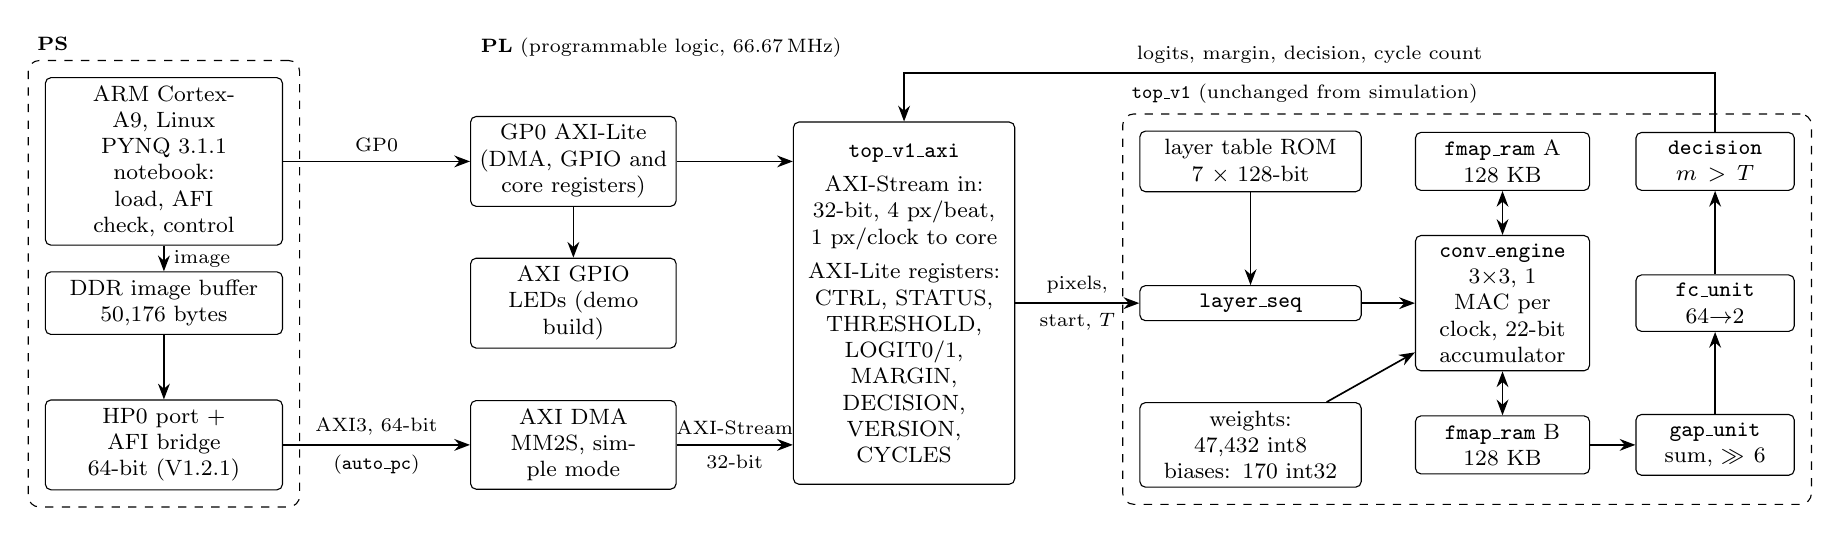
\begin{tikzpicture}[
  font=\footnotesize,
  blk/.style={draw, rounded corners=2pt, align=center, fill=white, inner sep=3pt, text width=#1},
  blk/.default={2.4cm},
  grp/.style={draw, dashed, rounded corners=4pt, inner sep=6pt},
  arr/.style={-{Stealth[length=2mm]}, semithick},
  lab/.style={font=\scriptsize, align=center}]
% processing system
\node[blk=2.8cm] (arm) at (1.6,4.1) {ARM Cortex-A9, Linux\\PYNQ 3.1.1 notebook:\\load, AFI check, control};
\node[blk=2.8cm] (ddr) at (1.6,2.3) {DDR image buffer\\50,176 bytes};
\node[blk=2.8cm] (hp0) at (1.6,0.5) {HP0 port + AFI bridge\\64-bit (V1.2.1)};
% interconnect, DMA, GPIO
\node[blk] (gp0) at (6.8,4.1) {GP0 AXI-Lite\\(DMA, GPIO and\\core registers)};
\node[blk] (gpio) at (6.8,2.3) {AXI GPIO\\LEDs (demo build)};
\node[blk] (dma) at (6.8,0.5) {AXI DMA\\MM2S, simple mode};
% wrapper
\node[blk=2.6cm, minimum height=4.6cm] (wrap) at (11.0,2.3)
  {\code{top\_v1\_axi}\\[3pt] AXI-Stream in:\\32-bit, 4 px/beat,\\1 px/clock to core\\[3pt] AXI-Lite registers:\\CTRL, STATUS,\\THRESHOLD, LOGIT0/1,\\MARGIN, DECISION,\\VERSION, CYCLES};
% core
\node[blk=2.6cm] (lt) at (15.4,4.1) {layer table ROM\\7 $\times$ 128-bit};
\node[blk=2.6cm] (seq) at (15.4,2.3) {\code{layer\_seq}};
\node[blk=2.6cm] (rom) at (15.4,0.5) {weights: 47,432 int8\\biases: 170 int32};
\node[blk=2.0cm] (fa) at (18.6,4.1) {\code{fmap\_ram} A\\128 KB};
\node[blk=2.0cm] (conv) at (18.6,2.3) {\code{conv\_engine}\\3$\times$3, 1 MAC per\\clock, 22-bit\\accumulator};
\node[blk=2.0cm] (fb) at (18.6,0.5) {\code{fmap\_ram} B\\128 KB};
\node[blk=1.8cm] (dec) at (21.3,4.1) {\code{decision}\\ $m > T$};
\node[blk=1.8cm] (fc) at (21.3,2.3) {\code{fc\_unit}\\64$\to$2};
\node[blk=1.8cm] (gap) at (21.3,0.5) {\code{gap\_unit}\\sum, $\gg 6$};
% groups
\node[lab, anchor=west] at (5.5,5.55) {\textbf{PL} (programmable logic, 66.67\,MHz)};
\node[grp, fit=(arm)(hp0), label={[lab, anchor=south west]north west:\textbf{PS}}] {};
\node[grp, fit=(lt)(rom)(dec)(gap), label={[lab, anchor=south west]north west:\textbf{\code{top\_v1}} (unchanged from simulation)}] (core) {};
% arrows
\draw[arr] (arm) -- node[lab, right] {image} (ddr);
\draw[arr] (ddr) -- (hp0);
\draw[arr] (hp0) -- node[lab, above] {AXI3, 64-bit} node[lab, below] {(\code{auto\_pc})} (dma);
\draw[arr] (arm) -- node[lab, above] {GP0} (gp0);
\draw[arr] (gp0) -- (gpio);
\draw[arr] (gp0.east) -- (gp0.east -| wrap.west);
\draw[arr] (dma.east) -- node[lab, above] {AXI-Stream} node[lab, below] {32-bit} (dma.east -| wrap.west);
\draw[arr] (wrap.east |- seq) -- node[lab, above] {pixels,} node[lab, below] {start, $T$} (seq);
\draw[arr] (lt) -- (seq);
\draw[arr] (seq) -- (conv);
\draw[arr] (rom) -- (conv);
\draw[arr, {Stealth[length=2mm]}-{Stealth[length=2mm]}] (fa) -- (conv);
\draw[arr, {Stealth[length=2mm]}-{Stealth[length=2mm]}] (fb) -- (conv);
\draw[arr] (fb) -- (gap);
\draw[arr] (gap) -- (fc);
\draw[arr] (fc) -- (dec);
\draw[arr] (dec.north) -- ++(0,0.75) -| node[lab, pos=0.25, above] {logits, margin, decision, cycle count} (wrap.north);
\end{tikzpicture}}
\caption{FLASH V1 on the Zynq-7020. The ARM core only moves data and polls registers, and all
inference runs in the programmable logic (PL). The input lands in buffer A, the layers alternate
between A and B, and GAP reads conv5's output from B. V1.2.1 runs the HP0 bridge and the DMA's
memory side at 64 bits (Section~\ref{sec:afi}).}
\label{fig:arch}
\end{figure*}

Figure~\ref{fig:arch} shows the system. The ARM core copies an image into a DMA buffer, writes
the threshold and a start bit, starts an AXI DMA \cite{pg021} in simple mode, polls a status
register, and reads back two logits, the margin, the decision and a cycle count.

\textit{The core.} \code{layer\_seq} walks a ROM of layer descriptors, one 128-bit word per
layer. Each holds the operation, kernel, stride and padding (4 bits each); input and output
channels, heights and widths (12 bits each); the shift (6 bits); and the weight and bias base
addresses (20 and 10 bits). It starts the right unit, swaps the two feature-map buffers between
layers and streams the GAP input. \code{conv\_engine} is shared by all five convolutions. It is
pipelined as operand multiplexer, register, multiplier, register and accumulator, and does one
MAC per clock. Padding is implemented as a gated read: an out-of-image tap contributes zero, so
no padded frame is stored. \code{gap\_unit} keeps 64 running sums, \code{fc\_unit} computes two
32-bit logits, and \code{decision} compares the margin with a run-time threshold register.

\textit{Scaling from 28$\times$28 to 224$\times$224.} The audited predecessor (v0) was a fixed
28$\times$28 design with one hand-written module per stage. Its classifier flattened a
4$\times$14$\times$14 map into a 784$\to$16 dense layer, so 99.7\% of its 12,634 parameters sat
in layers whose size grows with the image. At 224$\times$224 its first dense layer alone would
need 802,816 weights. In V1, moving from 28$\times$28 (stage V1.1) to 224$\times$224 (V1.2)
needed only new memory files (weights, biases, layer table) and one RTL change: the feature-map
buffers grew from 64\,KB to 128\,KB, because conv1's output is 8$\times$112$\times$112 = 100,352
bytes. The descriptor layout is identical at both sizes. MACs per image grow from 227,360 to
12,192,896, a factor of 53.6. That is less than the factor of 64 in pixels, because the small
maps at 28$\times$28 round up (7$\to$4$\to$2$\to$1). In synthesis of the core alone, block RAM
grows from 48.5 to 80.5 tiles. The convolution's address arithmetic ($c\cdot h\cdot w + y\cdot w
+ x$, a DSP multiply-add into the block-RAM address) is the critical path at both sizes.

\textit{The AXI wrapper.} \code{top\_v1\_axi} accepts the image as 32-bit AXI-Stream beats,
four pixels per beat, 12,544 beats per image, and feeds the core one pixel per clock. It
reproduces the exact drive sequence of the simulation testbench: threshold, all 50,176 pixels,
one idle cycle, one start pulse. It exposes the registers of Fig.~\ref{fig:arch}, with VERSION =
0xF1A50102 and CYCLES counting core clocks from start to result.

% ------------------------------------------------------------------------------------------
\section{Verification Methodology}\label{sec:verif}

Correctness is established by three links, each an exact comparison of integers with no
tolerance.
\begin{enumerate}
\item \textit{Trained network = golden model.} The golden model is an independent NumPy program
in int64 that reads only the exported files. It gives logits identical to the training framework
on all 4,003 test images, with 0 mismatches on every intermediate tensor of the 244 verification
images.
\item \textit{Golden model = RTL.} The simulator dumps every layer's output and a script compares
it with the golden model, so a mismatch points to one layer. At 224$\times$224, 16 of 16 images
and 12 of 12 per-layer traces are exact in Vivado xsim. The AXI wrapper passes a 33-check
testbench with varied bus timing and error cases. An independent audit re-ran the golden model
against all 244 vectors and 60 traces of both stages, with 0 mismatches.
\item \textit{RTL = board.} The board compares logit0, logit1, margin and decision with the
expected files on all 244 images (Section~\ref{sec:eval}).
\end{enumerate}

\textit{Unbiased vectors.} The 244 verification images are a seeded, balanced slice of the test
split, 122 pneumonia and 122 not. They were drawn without looking at the model's confidence, and
the model misclassifies 70 of them at $T$. The hardware has to reproduce these errors as well,
and an exact match of 32-bit logits on such images is very unlikely to occur by chance. The
hackathon prototype from which FLASH descends was tested by comparing one decision bit on eight
images that the model classified confidently, and three datapath defects remained undetected
across its five versions.

\textit{Defect ledger.} Table~\ref{tab:bugs} lists the technical defects found in all phases,
numbered as in the project's ledger. Defects 11 and 15 would have produced a device that gives
wrong answers without any error message. Two process problems are not in the table: an early
version of the documentation overstated the test coverage (12), and the export manifest records
hashes for only 3 of the 313 memory files of each stage (13, still open).

\begin{table}[t]
\caption{Technical defects found, all phases}
\label{tab:bugs}
\centering\footnotesize
\begin{tabular}{@{}p{0.55cm}p{4.6cm}p{2.5cm}@{}}
\toprule
\# & Defect & Found by \\
\midrule
1--5 & v0 (28$\times$28): line buffer read a pixel before it was written; windows centred one row
early; max-pool sampled block RAM a clock early; dense-layer pointer off by one; testbench
drove inputs on the sampling edge & golden-model tensor diff \\
6 & \code{gap\_unit} testbench raced the DUT & isolated reproduction \\
7 & conv and FC assumed 2-cycle reads; RAM had 1 & integration sweep \\
8 & sequencer needed two start pulses & integration sweep \\
9 & 64\,KB buffer too small for conv1 at 224 & first 224 simulation \\
10 & testbench timeout too short; literal wrapped & simulation \\
11 & synthesis loaded the 28$\times$28 weights through RTL defaults & synthesis log audit \\
14 & wrapper testbench sent a beat twice & first xsim run \\
15 & HP0 bridge 64-bit, design 32-bit & board, then offline model search \\
\bottomrule
\end{tabular}
\end{table}

% ------------------------------------------------------------------------------------------
\section{Implementation}\label{sec:impl}

The design targets the xc7z020clg400-1 with Vivado 2022.2. The block design holds the processing
system, the AXI DMA (read channel only), \code{top\_v1\_axi} as a module reference, a reset
block, and in one variant an AXI GPIO for the board LEDs. The DMA reaches DDR through the HP0
port. Vivado does not connect the AXI4 DMA directly to the AXI3 port, so a protocol converter
sits between them.

\textit{Clock.} The fabric clock is 66.67\,MHz (1000\,MHz/15). The processing system cannot
synthesise 75\,MHz exactly (a 75\,MHz request gives 76.92\,MHz), and the next lower frequency,
71.43\,MHz, failed post-route timing with WNS $-0.925$\,ns. At 66.67\,MHz the critical path, from
the convolution's address register through two DSP slices and one LUT into a block-RAM address
pin, takes 13.786\,ns of the 15\,ns budget, 70\% of it logic. The RTL was frozen for the board
work, so we accepted the lower clock; pipelining that path is a V2 item.

Table~\ref{tab:impl} gives the post-route results. V1.2.1 differs from V1.2 only in the HP0 and
DMA data width, and the LED variant adds the GPIO. The accelerator's netlist is identical in all
three: its 2,274 memory-initialisation lines match.

\begin{table}[t]
\caption{Post-route results, xc7z020 at 66.67\,MHz}
\label{tab:impl}
\centering\footnotesize
\setlength{\tabcolsep}{3.5pt}
\begin{tabular}{@{}lrrr@{}}
\toprule
 & V1.2 & V1.2.1 & V1.2.1-LED \\
 & (HP0 32-bit) & (HP0 64-bit) & \\
\midrule
WNS / WHS (ns)\meas & +0.206/+0.024 & +0.314/+0.030 & +0.344/+0.025 \\
Failing endpoints\meas & 0/15,320 & 0/15,451 & 0/15,704 \\
LUT\meas & 3,818 & 3,864 (7.3\%) & 3,947 \\
Flip-flops\meas & 4,745 & 4,766 (4.5\%) & 4,899 \\
BRAM tiles\meas & 81.5 & 82 (58.6\%) & 82 \\
DSP slices\meas & 14 & 14 (6.4\%) & 14 \\
Power, total (W)\synest & 1.492 & 1.494 & 1.499 \\
\quad of which PS7 (W)\synest & 1.256 & 1.256 & 1.256 \\
\bottomrule
\end{tabular}
\end{table}

Block RAM, mostly the two 128\,KB feature-map buffers, is the only substantial resource. Of the
3,864 LUTs of V1.2.1, the accelerator uses 2,758. Power is a vector-less Vivado estimate
(confidence Medium for the first two builds and Low for the LED build), and 84\% of it is the
processing system.

% ------------------------------------------------------------------------------------------
\section{Board Evaluation}\label{sec:eval}

The board runs PYNQ 3.1.1 \cite{pynq}. A notebook loads the bitstream, checks the version
register, the fabric clock and the AFI setting, then runs all 244 verification images and writes
a CSV file and a summary to the evidence folder.

\textit{Bit-exactness.} Table~\ref{tab:runs} lists the runs of 2026-10-09. On every image of every
run, CYCLES was 12,196,126 and the error bit was never set. Runs 1 and 3 wrote byte-identical CSV
files, and run 2 equals the failing board run of the previous day image by image.

\begin{table}[t]
\caption{Board runs, 244 images each}
\label{tab:runs}
\centering\footnotesize
\setlength{\tabcolsep}{3pt}
\begin{tabular}{@{}llcrr@{}}
\toprule
Run & Bitstream & AFI bit 0 & Bit-exact\meas & TP/FN/TN/FP\meas \\
\midrule
1 & V1.2.1 & 0 & 244/244 & 117/5/57/65 \\
2 & V1.2 (32-bit) & 0 & 0/244 & 118/4/56/66 \\
3 & V1.2 (32-bit) & 0$\to$1 & 244/244 & 117/5/57/65 \\
demo & V1.2.1-LED & 0 & 244/244 & 117/5/57/65 \\
\bottomrule
\end{tabular}
\end{table}

\textit{Accelerator metrics.} Table~\ref{tab:metrics} gives the usual figures of merit. The
12,192,896 MACs take 12,196,126 cycles. The remaining 3,230 cycles are the GAP stream (3,136) and
about 94 cycles of sequencing and pipeline drain, so the engine is busy with MACs in 99.97\% of
its cycles. With one MAC per clock the absolute performance is low. The FPGA is 3.6 to 4.1 times
faster than the same NumPy code on the board's ARM core, but a desktop PC runs that code in
8.7\,ms. The ARM baseline is unoptimised int64 NumPy on one core.

\begin{table}[t]
\caption{Accelerator metrics, V1.2.1 at 66.67\,MHz. PL power is the chip estimate minus the
PS7 share}
\label{tab:metrics}
\centering\footnotesize
\setlength{\tabcolsep}{3pt}
\begin{tabular}{@{}lr@{}}
\toprule
Latency, compute\meas & 182.94\,ms \\
Latency, end to end\meas & 184.73\,ms \\
Throughput, compute / end to end\deriv & 5.47 / 5.41 img/s \\
Work per image (2 ops/MAC)\deriv & 24.39\,MOP \\
Achieved / peak (1 MAC/clock)\deriv & 0.13330 / 0.13333\,GOP/s \\
MAC-cycle efficiency\deriv & 99.97\% \\
DSP / BRAM tiles / LUT\meas & 14 / 82 / 3,864 \\
Power, chip / PL\synest & 1.494 / 0.238\,W \\
Energy per image, chip / PL\deriv & 273.3 / 43.5\,mJ \\
Efficiency, chip / PL\deriv & 0.089 / 0.56\,GOP/s/W \\
\midrule
PC (i7-13650HX), NumPy int64\meas & 8.7\,ms \\
Board ARM Cortex-A9, same code\meas & 665--744\,ms \\
Board FPGA, compute / end to end\meas & 182.94 / 184.73\,ms \\
\bottomrule
\end{tabular}
\end{table}

\textit{Classification on the 244.} The board's own outputs give a sensitivity of 0.959 (Wilson
0.908--0.982), a specificity of 0.467 (0.381--0.555), PPV 0.643, NPV 0.919 and an AUROC of 0.837
(bootstrap 0.785--0.884, 2,000 resamples), consistent with the test-set AUROC. Of the 70 errors,
65 are false positives and 5 are false negatives, which matches a threshold chosen for at least
90\% sensitivity. The five false negatives have margins from $-736$ to $-670$, all within 90 of
$T$.

\begin{figure}[t]
\centering
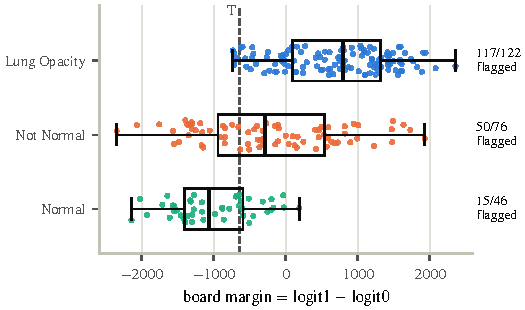
\includegraphics[width=\columnwidth]{figures/fig_margins_by_class.pdf}
\caption{Board margins on the 244 images by RSNA class (measured, board run 1). Dots are images,
boxes show the quartiles and the median, and the dashed line is $T=-646$. Two thirds of the
``Not Normal'' negatives lie above $T$.}
\label{fig:class}
\end{figure}

Figure~\ref{fig:class} shows where the false positives come from. RSNA's negative class mixes
``Normal'' with ``No Lung Opacity / Not Normal''. Of the 76 Not-Normal negatives, 50 are flagged
(65.8\%), against 15 of the 46 Normal ones (32.6\%). Their median margins, $-284.5$ and $-1061$,
lie on opposite sides of $T$. Figure~\ref{fig:subgroup} shows the same pattern on the full test
set, where pneumonia against Normal scores 0.936 and against Not Normal 0.738.

\begin{figure}[t]
\centering
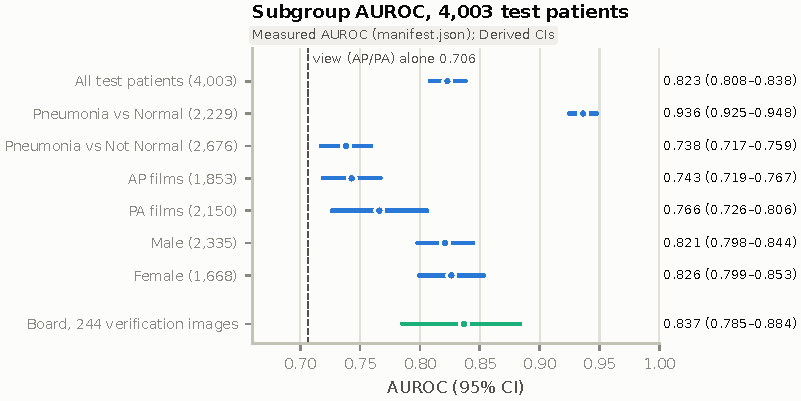
\includegraphics[width=\columnwidth]{figures/fig_subgroup_auroc.pdf}
\caption{Test-set AUROC by subgroup (measured, manifest of the training run). Intervals are the
bootstrap for all test patients and for the board's 244 images, and Hanley--McNeil
\cite{hanley1982} otherwise (derived), which overall gives a slightly wider 0.805--0.840. The
dashed line is the AUROC of the radiographic projection alone.}
\label{fig:subgroup}
\end{figure}

The subgroup analysis also exposes a shortcut. The projection alone, AP (taken at the bedside,
often of sicker patients) or PA, predicts the label with an AUROC of 0.706. Within AP films or
within PA films the model scores only 0.743 and 0.766, so part of its overall 0.823 comes from
the projection. Men and women score the same within error (0.821 and 0.826).

\begin{figure}[t]
\centering
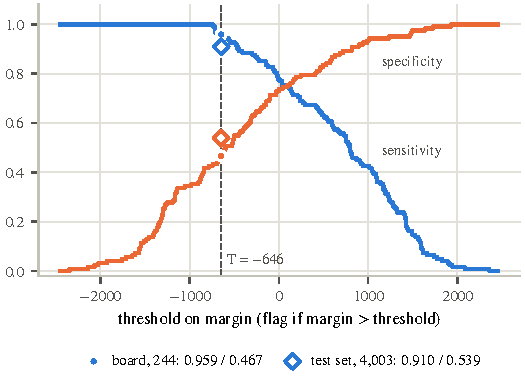
\includegraphics[width=\columnwidth]{figures/fig_operating_characteristic.pdf}
\caption{Sensitivity and specificity against the threshold, from the 244 board margins
(derived). Diamonds mark the test-set operating point. The plot is illustrative only, because
$T$ was fixed on validation data.}
\label{fig:oc}
\end{figure}

\begin{figure}[t]
\centering
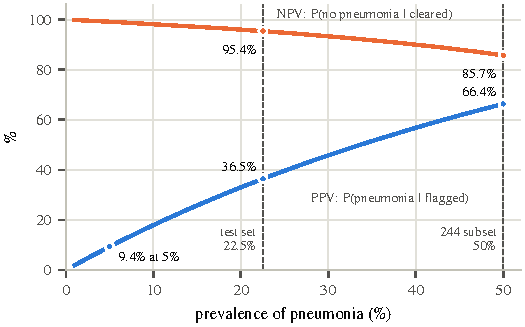
\includegraphics[width=\columnwidth]{figures/fig_ppv_npv_prevalence.pdf}
\caption{PPV and NPV at the test operating point (821 of 902 positives flagged, 1,671 of 3,101
negatives cleared) as the prevalence varies (derived).}
\label{fig:prev}
\end{figure}

Figure~\ref{fig:oc} shows the trade-off that a different $T$ would give, and
Figure~\ref{fig:prev} shows how a positive result should be read in deployment. At the test
prevalence of 22.5\% the PPV is 36.5\% and the NPV 95.4\%. At a prevalence of 5\% the PPV falls
to 9.4\%, about one positive in eleven, while the NPV rises to 99.1\%. The 244 subset is balanced
by construction, so its PPV of 0.643 does not describe deployment. A negative result is
therefore informative at realistic prevalences, whereas a positive result is best used to
prioritise a radiograph for reading.

% ------------------------------------------------------------------------------------------
\section{Case Study: A Fault Only the Board Could Show}\label{sec:afi}

\begin{figure*}[t]
\centering
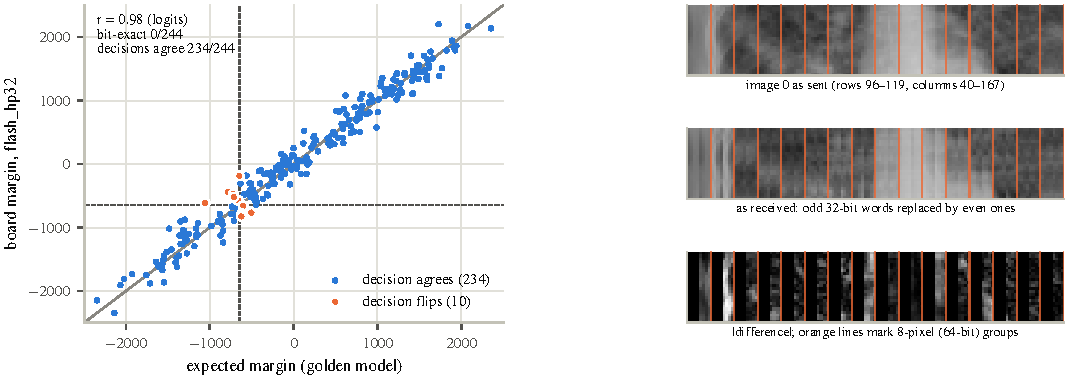
\includegraphics[width=\textwidth]{figures/fig_afi_case.pdf}
\caption{Left: the first board run, V1.2, against the expected margins (measured). The logits
correlate at $r=0.98$ and 234 of 244 decisions agree, yet no image is bit-exact. Right: a crop of
image 0 as sent and as the PL received it under the dup\_even model (derived). Each 64-bit group
keeps its first four pixels and repeats them, a mild horizontal blur that GAP largely tolerates.}
\label{fig:afi}
\end{figure*}

\textit{Symptom.} The first V1.2 bitstream produced no bit-exact result (0/244). The other
indicators were normal (Fig.~\ref{fig:afi}). The logits correlated with the expected values at
0.98, and 234 of 244 decisions agreed. The results were identical at 25, 50 and 66.67\,MHz, which
excludes a timing failure, and repeated runs and soft resets gave identical outputs. The DMA
reported no error. A test that compared only decisions would have accepted this hardware.

\textit{Offline localisation.} Instead of modifying the RTL, we used the golden model to
interpret synthetic probe images sent to the board. Constant images and an image constant along
each row came back exact, while a ramp along each row did not, which pointed at the order of
pixels within a row. We then searched candidate corruptions (byte orders within a beat, row
shifts, flips, block reversals, beat permutations and padding variants) for one that reproduces
every board output. Only one candidate did: each odd 32-bit input word, four pixels, is replaced
by the even word before it (``dup\_even''). It reproduces the board on 244 of 244 images and 24 of
24 probes, where the unmodified golden model matches only 12 of the 24 probes. A word pair never
crosses a 224-pixel row, which is why the row-constant probes were unaffected.

\textit{Prediction before observation.} For the second probe set, the outputs predicted by the
model were recorded before the board's results were examined. Two single-pixel probes
discriminate. For a bright pixel at (1,0), dup\_even predicts $(-349, 102, 451)$ for (logit0,
logit1, margin), and the golden model predicts the all-zero image's result, $(-375, 106, 481)$.
For a bright pixel at (223,223) the roles are exchanged: dup\_even predicts the all-zero result
and the golden model $(-386, 114, 500)$. The board matched the dup\_even predictions exactly.

\textit{Mechanism and intervention.} The DMA reads DDR through the HP0 port, whose AFI bridge has
its own width setting, bit 0 of its RDCHAN\_CTRL register \cite{ug585}. V1.2 used a 32-bit HP0,
but PYNQ boots the processing system with the AFI in 64-bit mode and does not run the design's
own initialisation code, so each 32-bit read returned the low half of a 64-bit word, the even
word. On one boot, the 32-bit bitstream gave 0/244 (run 2), and after that single bit was written
from 0 to 1 it gave 244/244 (run 3). No other setting changed between the two runs, which
identifies the register bit as the cause.

\textit{Fix.} V1.2.1 makes HP0 and the DMA's memory side 64-bit, which matches PYNQ's default and
needs no register write (run 1). Every board notebook now compares the AFI setting with the
bitstream's hardware description and refuses to run on a mismatch. The simulations drove the
stream directly and did not model the processor's memory path, so they could not reveal this
fault. Because the network tolerates this kind of input corruption, its decisions stayed mostly
correct while every logit was wrong, and the fault was detected only because the board's logits
were compared with the reference.

% ------------------------------------------------------------------------------------------
\section{Discussion: Clinical Readiness and the Regulatory Gap}\label{sec:disc}

FLASH demonstrates exact hardware execution of the integer network; whether the network is
clinically useful is a separate question that this work does not answer. An AUROC of 0.82 on one
public adult dataset is research grade. The model separates pneumonia from normal lungs well, but
at $T$ its test-set specificity is 33.4\% against other abnormalities, compared with 81.3\%
against normal lungs, and a screener in a real clinic will see such abnormalities constantly.
Part of its score comes from the projection, which partly reflects how unwell the patient was when
the film was ordered, since AP films are often taken at the bedside. This is the kind of shortcut
that \cite{zech2018,degrave2021,geirhos2020} warn about.

Reporting guidelines make the gaps concrete. CLAIM \cite{mongan2020claim} and TRIPOD+AI
\cite{collins2024tripodai} ask authors to state, among other things, the intended use, how the
model was validated, including on external data, and how it performs across subgroups. FLASH
reports subgroups and a locked, validation-chosen operating point, but it has no external or
paediatric validation, no comparison with radiologists and no prospective data. Pneumonia
mortality is concentrated in children \cite{who2022pneumonia}, while RSNA contains adults.

\textit{Threats to validity.} The model was trained and tested on one adult dataset from a single
source, so its accuracy on other populations, scanners and on children is unknown. The board
results cover 244 of the 4,003 test images. The test-set accuracy is the golden model's, and its
equality with the board on the remaining images is inferred from the 244. The power figures are
vector-less Vivado estimates and have not been measured. The ARM comparison uses unoptimised
NumPy code on one core, so the reported speed-up over the ARM is an upper bound on what the FPGA
adds.

Regulation adds process on top of evidence. A device would need a software life-cycle process
(IEC 62304 \cite{iec62304}), risk management (ISO 14971 \cite{iso14971}) and a quality
management system (ISO 13485 \cite{iso13485}). The FDA's action plan \cite{fda2021aiml} describes
how AI/ML-based software that changes over time should be managed. Bit-exactness addresses one
narrow part of this process, verification. It shows that the deployed hardware computes the
validated function on the tested inputs, and a change of threshold is a register value rather
than a new model. It does not address clinical validity, and FLASH is therefore a research
prototype and not a medical device.

% ------------------------------------------------------------------------------------------
\section{Future Work (V2)}\label{sec:v2}

The project pauses after V1. Three items would move the remaining software-based results onto
the board:
\begin{itemize}
\item \textit{A board run on all 4,003 test images.} The 4,003-image accuracy is the golden
model's, bit-exact to the board on 244 images; a full board run (about 12 minutes of compute)
would make it the board's own output.
\item \textit{Measured board power.} The power figures so far are Vivado estimates.
\item \textit{DICOM end to end on the board.} The DICOM preprocessing has only been verified on
the PC.
\end{itemize}

Beyond those, the model needs a clinical operating point: explicit treatment of the Not-Normal
class, an analysis per projection, and a threshold chosen on validation data for a stated
specificity as well as sensitivity. Since $T$ is a register, none of this needs a hardware change.

\begin{figure}[t]
\centering
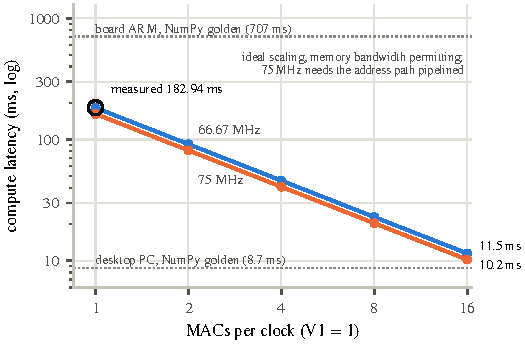
\includegraphics[width=\columnwidth]{figures/fig_v2_projection.pdf}
\caption{Projected compute latency against MACs per clock, derived from the measured cycle
count. The projection assumes ideal scaling of the MAC cycles, fixed non-MAC cycles and
sufficient memory bandwidth; 75\,MHz assumes a pipelined address path.}
\label{fig:v2}
\end{figure}

On the hardware side, only 14 of 220 DSP slices are used. Several MACs per clock need wider or
parallel feature-map reads, since the engine now reads one byte per clock, and a line-buffer
window generator is already built and tested for this. Figure~\ref{fig:v2} projects the gain. At
16 MACs per clock the compute time would be 11.5\,ms at 66.67\,MHz and 10.2\,ms at 75\,MHz, still
above the desktop PC's 8.7\,ms. Any advantage of the FPGA in V2 therefore has to come from power,
determinism and cost as well as speed, which is why measured power is among the items above.

% ------------------------------------------------------------------------------------------
\section{Conclusion}

FLASH runs a 224$\times$224 integer CNN for pneumonia screening entirely in the programmable logic
of a Zynq-7020 and reproduces an independent reference model bit for bit on all 244 verification
images, across three bitstreams. A layer-table-driven engine let the same Verilog scale from
28$\times$28 to 224$\times$224 with new memory files and one buffer size. A board-only bus-width
fault left 234 of 244 decisions intact while corrupting every logit; logit-level comparison
detected it, the golden model localised it offline, and a one-bit intervention confirmed it. The
model's accuracy is modest, and its two failure modes, the Not-Normal confusion and the
projection shortcut, are reported with it.

\section*{Data and Code Availability}

The RTL, Vivado scripts, board notebooks, bitstreams, hardware reports, raw board evidence and the
scripts that derive every number and figure in this paper are available at
\url{https://github.com/Karthik-Flash/ProjectFlash} (tag \code{v1.2.1-hw}). The data are those of
the RSNA Pneumonia Detection Challenge on Kaggle \cite{rsnadata}, described by Shih \textit{et al.}
\cite{shih2019rsna}, and the radiographs originate from the NIH Chest X-ray dataset
\cite{nihdata,wang2017chestxray8}. The verification vectors are regenerated from the data by the
project's training notebook with a fixed seed.

\section*{Ethics and Data Licence}

This study used only de-identified, publicly available radiographs and annotations from the RSNA
Pneumonia Detection Challenge \cite{rsnadata,shih2019rsna}, under the competition's data-use rules
and RSNA's terms of use. RSNA's terms permit research use and prohibit any attempt to identify or
contact the subjects. The NIH Clinical Center is the provider of the radiographs. No data were
collected from patients for this work. The paper reproduces no radiographs; the figures in the
repository that show radiographs carry the attribution that the terms require.

\section*{Acknowledgment}

The first FLASH prototype was developed for the AMD FPGA Hackathon 2026, held at BITS Pilani,
Hyderabad Campus, in March 2026 and organised by IEEE BPHC, the IEEE Student Branch of BITS
Pilani, Hyderabad Campus. FLASH placed 5th, and we thank the organisers. We acknowledge the NIH
Clinical Center as the provider of the chest radiographs, and the RSNA and the Society of
Thoracic Radiology for the pneumonia annotations.

\begin{thebibliography}{32}

\bibitem{who2022pneumonia}
World Health Organization, ``Pneumonia in children,'' Fact sheet, Nov. 2022. [Online].
Available: \url{https://www.who.int/news-room/fact-sheets/detail/pneumonia}

\bibitem{wang2017chestxray8}
X.~Wang, Y.~Peng, L.~Lu, Z.~Lu, M.~Bagheri, and R.~M. Summers, ``{ChestX-Ray8}:
Hospital-scale chest {X}-ray database and benchmarks on weakly-supervised classification and
localization of common thorax diseases,'' in \emph{Proc. IEEE Conf. Computer Vision and Pattern
Recognition (CVPR)}, 2017, pp. 3462--3471.

\bibitem{rajpurkar2017chexnet}
P.~Rajpurkar, J.~Irvin, K.~Zhu, B.~Yang, H.~Mehta, T.~Duan, D.~Ding, A.~Bagul, C.~Langlotz,
K.~Shpanskaya, M.~P. Lungren, and A.~Y. Ng, ``{CheXNet}: Radiologist-level pneumonia detection
on chest {X}-rays with deep learning,'' arXiv:1711.05225, 2017. [Online]. Available:
\url{https://arxiv.org/abs/1711.05225}

\bibitem{shih2019rsna}
G.~Shih, C.~C. Wu, S.~S. Halabi, M.~D. Kohli, L.~M. Prevedello, T.~S. Cook, A.~Sharma
\emph{et~al.}, ``Augmenting the National Institutes of Health chest radiograph dataset with
expert annotations of possible pneumonia,'' \emph{Radiology: Artificial Intelligence}, vol.~1,
no.~1, p. e180041, 2019.

\bibitem{kermany2018}
D.~S. Kermany, M.~Goldbaum, W.~Cai, C.~C.~S. Valentim, H.~Liang, S.~L. Baxter \emph{et~al.},
``Identifying medical diagnoses and treatable diseases by image-based deep learning,''
\emph{Cell}, vol.~172, no.~5, pp. 1122--1131.e9, 2018.

\bibitem{yang2023medmnist}
J.~Yang, R.~Shi, D.~Wei, Z.~Liu, L.~Zhao, B.~Ke, H.~Pfister, and B.~Ni, ``{MedMNIST} v2: A
large-scale lightweight benchmark for {2D} and {3D} biomedical image classification,''
\emph{Scientific Data}, vol.~10, p.~41, 2023.

\bibitem{zech2018}
J.~R. Zech, M.~A. Badgeley, M.~Liu, A.~B. Costa, J.~J. Titano, and E.~K. Oermann, ``Variable
generalization performance of a deep learning model to detect pneumonia in chest radiographs: A
cross-sectional study,'' \emph{PLOS Medicine}, vol.~15, no.~11, p. e1002683, 2018.

\bibitem{degrave2021}
A.~J. DeGrave, J.~D. Janizek, and S.-I. Lee, ``{AI} for radiographic {COVID-19} detection selects
shortcuts over signal,'' \emph{Nature Machine Intelligence}, vol.~3, no.~7, pp. 610--619, 2021.

\bibitem{geirhos2020}
R.~Geirhos, J.-H. Jacobsen, C.~Michaelis, R.~Zemel, W.~Brendel, M.~Bethge, and F.~A. Wichmann,
``Shortcut learning in deep neural networks,'' \emph{Nature Machine Intelligence}, vol.~2,
no.~11, pp. 665--673, 2020.

\bibitem{jacob2018}
B.~Jacob, S.~Kligys, B.~Chen, M.~Zhu, M.~Tang, A.~Howard, H.~Adam, and D.~Kalenichenko,
``Quantization and training of neural networks for efficient integer-arithmetic-only
inference,'' in \emph{Proc. IEEE/CVF Conf. Computer Vision and Pattern Recognition (CVPR)},
2018, pp. 2704--2713.

\bibitem{lin2014nin}
M.~Lin, Q.~Chen, and S.~Yan, ``Network in network,'' in \emph{Proc. Int. Conf. Learning
Representations (ICLR)}, 2014. [Online]. Available: \url{https://arxiv.org/abs/1312.4400}

\bibitem{springenberg2015}
J.~T. Springenberg, A.~Dosovitskiy, T.~Brox, and M.~Riedmiller, ``Striving for simplicity: The
all convolutional net,'' in \emph{Proc. Int. Conf. Learning Representations (ICLR), Workshop
Track}, 2015. [Online]. Available: \url{https://arxiv.org/abs/1412.6806}

\bibitem{zhang2015}
C.~Zhang, P.~Li, G.~Sun, Y.~Guan, B.~Xiao, and J.~Cong, ``Optimizing {FPGA}-based accelerator
design for deep convolutional neural networks,'' in \emph{Proc. ACM/SIGDA Int. Symp.
Field-Programmable Gate Arrays (FPGA)}, 2015, pp. 161--170.

\bibitem{qiu2016}
J.~Qiu, J.~Wang, S.~Yao, K.~Guo, B.~Li, E.~Zhou, J.~Yu, T.~Tang, N.~Xu, S.~Song, Y.~Wang, and
H.~Yang, ``Going deeper with embedded {FPGA} platform for convolutional neural network,'' in
\emph{Proc. ACM/SIGDA Int. Symp. Field-Programmable Gate Arrays (FPGA)}, 2016, pp. 26--35.

\bibitem{umuroglu2017finn}
Y.~Umuroglu, N.~J. Fraser, G.~Gambardella, M.~Blott, P.~Leong, M.~Jahre, and K.~Vissers,
``{FINN}: A framework for fast, scalable binarized neural network inference,'' in \emph{Proc.
ACM/SIGDA Int. Symp. Field-Programmable Gate Arrays (FPGA)}, 2017, pp. 65--74.

\bibitem{duarte2018hls4ml}
J.~Duarte, S.~Han, P.~Harris, S.~Jindariani, E.~Kreinar, B.~Kreis, J.~Ngadiuba, M.~Pierini
\emph{et~al.}, ``Fast inference of deep neural networks in {FPGAs} for particle physics,''
\emph{Journal of Instrumentation}, vol.~13, no.~07, p. P07027, 2018.

\bibitem{sze2017}
V.~Sze, Y.-H. Chen, T.-J. Yang, and J.~S. Emer, ``Efficient processing of deep neural networks:
A tutorial and survey,'' \emph{Proceedings of the IEEE}, vol.~105, no.~12, pp. 2295--2329, 2017.

\bibitem{mongan2020claim}
J.~Mongan, L.~Moy, and C.~E. Kahn,~Jr., ``Checklist for artificial intelligence in medical
imaging ({CLAIM}): A guide for authors and reviewers,'' \emph{Radiology: Artificial
Intelligence}, vol.~2, no.~2, p. e200029, 2020.

\bibitem{collins2024tripodai}
G.~S. Collins, K.~G.~M. Moons, P.~Dhiman, R.~D. Riley, A.~L. Beam, B.~Van~Calster,
M.~Ghassemi, X.~Liu \emph{et~al.}, ``{TRIPOD+AI} statement: Updated guidance for reporting
clinical prediction models that use regression or machine learning methods,'' \emph{BMJ},
vol.~385, p. e078378, 2024.

\bibitem{wilson1927}
E.~B. Wilson, ``Probable inference, the law of succession, and statistical inference,''
\emph{Journal of the American Statistical Association}, vol.~22, no.~158, pp. 209--212, 1927.

\bibitem{efron1979}
B.~Efron, ``Bootstrap methods: Another look at the jackknife,'' \emph{The Annals of
Statistics}, vol.~7, no.~1, pp. 1--26, 1979.

\bibitem{hanley1982}
J.~A. Hanley and B.~J. McNeil, ``The meaning and use of the area under a receiver operating
characteristic ({ROC}) curve,'' \emph{Radiology}, vol.~143, no.~1, pp. 29--36, 1982.

\bibitem{iec62304}
\emph{{IEC} 62304:2006, Medical Device Software: Software Life Cycle Processes}, International
Electrotechnical Commission, 2006, Amendment 1, 2015. [Online]. Available:
\url{https://webstore.iec.ch/publication/6792}

\bibitem{iso14971}
\emph{{ISO} 14971:2019, Medical Devices: Application of Risk Management to Medical Devices},
International Organization for Standardization, 2019. [Online]. Available:
\url{https://www.iso.org/standard/72704.html}

\bibitem{iso13485}
\emph{{ISO} 13485:2016, Medical Devices: Quality Management Systems, Requirements for
Regulatory Purposes}, International Organization for Standardization, 2016. [Online].
Available: \url{https://www.iso.org/standard/59752.html}

\bibitem{fda2021aiml}
U.S. Food and Drug Administration, ``Artificial intelligence/machine learning ({AI/ML})-based
software as a medical device ({SaMD}) action plan,'' Center for Devices and Radiological
Health, Tech. Rep., Jan. 2021. [Online]. Available:
\url{https://www.fda.gov/media/145022/download}

\bibitem{rsnadata}
Radiological Society of North America, ``{RSNA} Pneumonia Detection Challenge,'' Kaggle
competition, 2018. [Online]. Available:
\url{https://www.kaggle.com/competitions/rsna-pneumonia-detection-challenge}

\bibitem{dicom}
National Electrical Manufacturers Association, \emph{Digital Imaging and Communications in
Medicine ({DICOM}) Standard, {NEMA} {PS3} / {ISO} 12052}. [Online]. Available:
\url{https://dicom.nema.org/medical/dicom/current/output/html/part01.html}

\bibitem{pg021}
AMD, \emph{{AXI DMA} {LogiCORE} {IP} Product Guide ({PG021}), v7.1}. [Online]. Available:
\url{https://docs.amd.com/r/en-US/pg021_axi_dma}

\bibitem{pynq}
AMD, ``{PYNQ}: Python productivity for adaptive computing platforms,'' open-source project.
[Online]. Available: \url{https://www.pynq.io/}

\bibitem{ug585}
Xilinx, Inc. (now AMD), \emph{Zynq-7000 {SoC} Technical Reference Manual ({UG585})},
Appendix~B, AFI registers. [Online]. Available:
\url{https://docs.amd.com/v/u/en-US/ug585-Zynq-7000-TRM}

\bibitem{nihdata}
NIH Clinical Center, ``{NIH} Chest X-ray Dataset,'' download site named in the RSNA terms of
use. [Online]. Available: \url{https://nihcc.app.box.com/v/ChestXray-NIHCC}

\end{thebibliography}

\end{document}